\documentclass{article}
\usepackage{amsmath, sfmath, multicol, tkz-euclide, array, enumerate, tcolorbox, tabularray}
\renewcommand{\familydefault}{\sfdefault}
\setlength{\parindent}{0cm}
\pagestyle{empty}
\usepackage[left=1in, top=0.5in, right=1in, bottom=0.5in]{geometry}
\tikzset{>=stealth}
\tcbset{colback=white}

\newcounter{example}[section]
\newenvironment{example}[1][]{\refstepcounter{example}\par\medskip
   {\color{red}\textbf{Example~\theexample. #1}}}{\medskip}

\begin{document}

\section*{Inequalities in One Triangle}

\begin{tcolorbox}[colframe=orange!70!white, coltitle=black, title=\textbf{Today I Can}]
\begin{enumerate}
    \item Write and solve inequalities for angles and sides of a triangle.
\end{enumerate}
\end{tcolorbox}
\smallskip 

\begin{center}
\emph{The longer the side of a triangle, the larger the angle opposite that side; and vice versa.}
\end{center}

\begin{example}
Put the angles of the triangle in order from least to greatest.
\newline

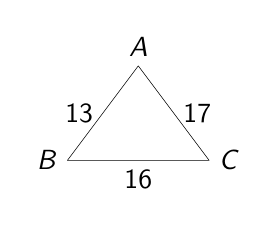
\begin{tikzpicture}[scale=0.6]
\tkzDefPoints{0/0/B, 3/0/C, 1.5/2/A}
\tkzDrawPolygon(A,B,C)
\tkzLabelPoints[left](B)
\tkzLabelPoints[above](A)
\tkzLabelPoints[right](C)
\tkzLabelSegment[left](A,B){13}
\tkzLabelSegment[below](B,C){16}
\tkzLabelSegment[right](A,C){17}
\end{tikzpicture}
\end{example}

\vspace{0.25in}

\begin{example}
If the perimeter of the triangle below is 47, Find the measure of the largest angle.
\newline

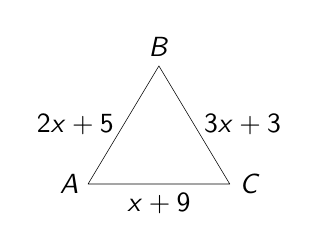
\begin{tikzpicture}[scale=0.6]
\tkzDefPoints{0/0/A, 3/0/C, 1.5/2.5/B}
\tkzDrawPolygon(A,B,C)
\tkzLabelPoints[left](A)
\tkzLabelPoints[above](B)
\tkzLabelPoints[right](C)
\tkzLabelSegment[left](A,B){$2x+5$}
\tkzLabelSegment[below](A,C){$x+9$}
\tkzLabelSegment[right](B,C){$3x+3$}
% \node at (1.5,0.5) {Perim = 47};
\end{tikzpicture}
\end{example}

\vfill 

\begin{example}
Put the sides of the triangle in order from shortest to longest. \newline

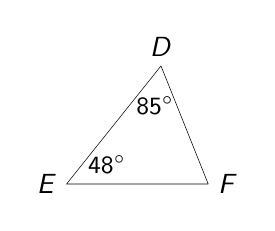
\begin{tikzpicture}[scale=0.6]
\tkzDefPoints{0/0/E, 3/0/F, 2/2.5/D}
\tkzDrawPolygon(E,D,F)
\tkzLabelPoints[left](E)
\tkzLabelPoints[above](D)
\tkzLabelPoints[right](F)
\tkzLabelAngle[pos=0.95](F,E,D){\small $48^\circ$}
\tkzLabelAngle[pos=0.85](E,D,F){\small $85^\circ$}
\end{tikzpicture}
\end{example}

\vspace{0.25in}

\begin{example}
List the sides of $\triangle ABC$ in order from shortest to longest given the following angle measures:
\[
m\angle A = 9x-4, \quad m\angle B = 4x-16, \quad m\angle C = 68-2x
\]
\end{example}

\vfill 
\newpage 

\begin{tcolorbox}[colframe=black!20!white, opacitybacktitle=0.1, coltitle=black, title=\textbf{Triangle Inequality Theorem}]
Any 2 sides of a triangle added together must be longer than the 3rd side.
\end{tcolorbox}

\bigskip 

\begin{example}
Can a triangle have sides with the given lengths? Explain.
\begin{multicols}{2}
\begin{enumerate}[(a)]
    \item 3 ft, 7 ft, 8 ft
    \item 5 ft, 10 ft, 15 ft
\end{enumerate}
\end{multicols}
\end{example}

\vspace{1in}

\begin{example}
Find the range of possible lengths for the third side in each.
\begin{enumerate}[(a)]
    \item Two sides of a triangle are 9 yd and 4 yd     \vspace{1.5in}
    \item Two sides of a triangle are 4 ft and 7 ft
\end{enumerate}
\end{example}


\end{document}
